\documentclass[compress]{beamer}

%\usepackage[latin1,utf8]{inputenc}

%\usepackage[utf8]{inputenc}
%\usepackage[utf8]{inputenc}
\usepackage[T1]{fontenc}
\usepackage[english]{babel}

\usetheme{shadow}
\usepackage{multirow}
\usepackage{tikz}
\usepackage{xcolor}
\usepackage{amsmath}
\usepackage{graphicx}
\usepackage{epstopdf}
\usepackage{textpos}
\usepackage{textcomp}
\usepackage{color, colortbl}
\usepackage{fancybox}
\usepackage{boxedminipage}
\usepackage{xcolor}
\usepackage{lipsum}
\usepackage{comment}
\usepackage{rotating}
\usepackage{xcolor}

\usepackage{epsfig}
\usepackage{amsmath,amssymb}
\usepackage{amsthm}
\usepackage{multirow}
\usepackage{graphicx}
\usepackage{boxedminipage}
\usepackage{latexsym}
\usepackage{subfigure}
\usepackage{wrapfig}
\usepackage{algorithm} 
\usepackage{appendixnumberbeamer}

\usepackage{framed}

\usetikzlibrary{shapes}
\usetikzlibrary{arrows}
\usetikzlibrary{automata}
\usepackage{algorithm}
\usepackage[noend]{algorithmic}
\usepackage{pifont}
\usepackage{fancybox}
\usepackage{listings}
\usepackage{changepage}

% Daniele
\usepackage{adjustbox}

\lstset{escapeinside={<@}{@>}}

% needed if you use oopdf2eps script :)
\epstopdfsetup{suffix=}

\beamertemplatenavigationsymbolsempty 

\title[BlueTracer:
a Robust API Tracer for Evasive Malware]{BlueTracer: \\
a Robust API Tracer for Evasive Malware}

\author[Simone Nicchi]
{
    \textbf{\textcolor{sapienza}{Simone Nicchi}\\~\\{\vspace{-0.5em}\em\textmd{Thesis Advisor: Prof. Camil Demetrescu \\ Thesis Co-Advisors: Dr. Daniele Cono D'Elia, Dr. Emilio Coppa} }\\~\\{Master of Science in Engineering in Computer Science}}\vspace{-2em}
}

%\pgfdeclareimage[height=1.6cm]{logo}{Immagini/sapienza}
%\logo{\centering \pgfuseimage{logo}} 

%\institute[Sapienza Universit\`{a} di Roma, Italy]
%{
  %\inst{1}%
  %Sapienza Universit\`{a} di Roma, Italy\\
  %\and
  %\vskip-2mm
  %\inst{2}%
  %Sapienza Universit\`{a} di Roma, Italy\\
%  \texttt{\space crisafulli.giu@gmail.com}
%}


%\date{\today}
\date{July 20, 2018}
\newcommand{\argmax}{\operatornamewithlimits{argmax}\limits}
\definecolor{forest}{RGB}{21,166,64}
\newcommand\mybox[2][]{\tikz[overlay]\node[ draw=forest, fill=blue!20,inner sep=2pt, anchor=text, rectangle, rounded corners=1mm, #1] {#2};\phantom{#2}}

\begin{document}

\definecolor{sapienza}{rgb}{0.50,0.14,0.20}
\definecolor{LightCyan}{rgb}{0.88,1,1}
\definecolor{Gray}{gray}{0.9}

\newcommand\darrow{\fontsize{36pt}{36pt}\selectfont{\begin{turn}{-90}\bf {\textcolor{sapienza}{\ding{224}}}\end{turn}}}
\newcommand\larrow{\fontsize{36pt}{36pt}\selectfont\bf {\textcolor{sapienza}{\ding{224}}}}
\newcommand\blarrow{\fontsize{36pt}{36pt}\selectfont{\begin{turn}{-135}\bf {\textcolor{sapienza}{\ding{224}}}\end{turn}}}

% insert page number
\newcommand*\oldmacro{}
\let\oldmacro\insertshortauthor% save previous definition
\renewcommand*\insertshortauthor{%
  \leftskip=.3cm% before the author could be a plus1fill ...
  \insertframenumber\,/\,\inserttotalframenumber\hfill\oldmacro}

\newcommand\emlarrow{%
        {\bf {\textcolor{sapienza}{\ding{224}}}}%
}

\setbeamercolor*{alerted text}{bg=white,fg=sapienza}
\setbeamercolor*{structure}{bg=white,fg=sapienza}

\setbeamercolor*{palette primary}{use=structure,fg=white,bg=sapienza}
\setbeamercolor*{palette secondary}{use=structure,fg=white}
\setbeamercolor*{palette tertiary}{use=structure,fg=white}
\setbeamercolor*{palette quaternary}{fg=black,bg=white}

\setbeamercolor*{sidebar}{use=structure,bg=structure.fg}
  
\setbeamercolor*{palette sidebar primary}{use=structure}
\setbeamercolor*{palette sidebar secondary}{fg=white}
\setbeamercolor*{palette sidebar tertiary}{use=structure}
\setbeamercolor*{palette sidebar quaternary}{fg=white}

\setbeamercolor*{titlelike}{parent=palette primary}

\setbeamercolor*{separation line}{}
\setbeamercolor*{fine separation line}{}


\setbeamercolor{frametitle}{fg=white,bg=sapienza!100}
\setbeamercolor{frametitle right}{fg=white,bg=sapienza!100}
\setbeamercolor{subsection in head/foot}{bg=sapienza}
\setbeamercolor{title in head/foot}{bg=sapienza}


% insert page number
%\newcommand*\oldmacro{}
%\let\oldmacro\insertshortauthor% save previous definition
%\renewcommand*\insertshortauthor{%
%  \leftskip=.3cm% before the author could be a plus1fill ...
%  \insertframenumber\,/\,\inserttotalframenumber\hfill\oldmacro}

\newcommand{\stt}{\small\tt}
\newcommand{\word}[1]{\fontsize{10.4}{10}\textsf{#1}}        % mention of word
\newcommand{\wordb}[2]{\fontsize{10.4}{10}\textsf{#1}$_#2$}        % mention of word
\newcommand{\wordc}[3]{\fontsize{10.4}{10}\textsf{#1}$_#2^#3$}        % mention of word
\newcommand{\wikipage}[1]{\textsc{#1}}        % mention of wikipage

\newcommand\tab[1][0.5cm]{\hspace*{#1}}

\begin{frame}
 
 \begin{figure}
     \centering
    \vspace{0.5cm}
     
\includegraphics[scale=.40]{image/sapienza.png}\\
    
 \end{figure}
 
\titlepage
\end{frame}

\section{Introduction}
\subsection{Malware Analysis}

\begin{frame}
    \frametitle{Malware: an increasingly significant problem }

    \begin{figure}
        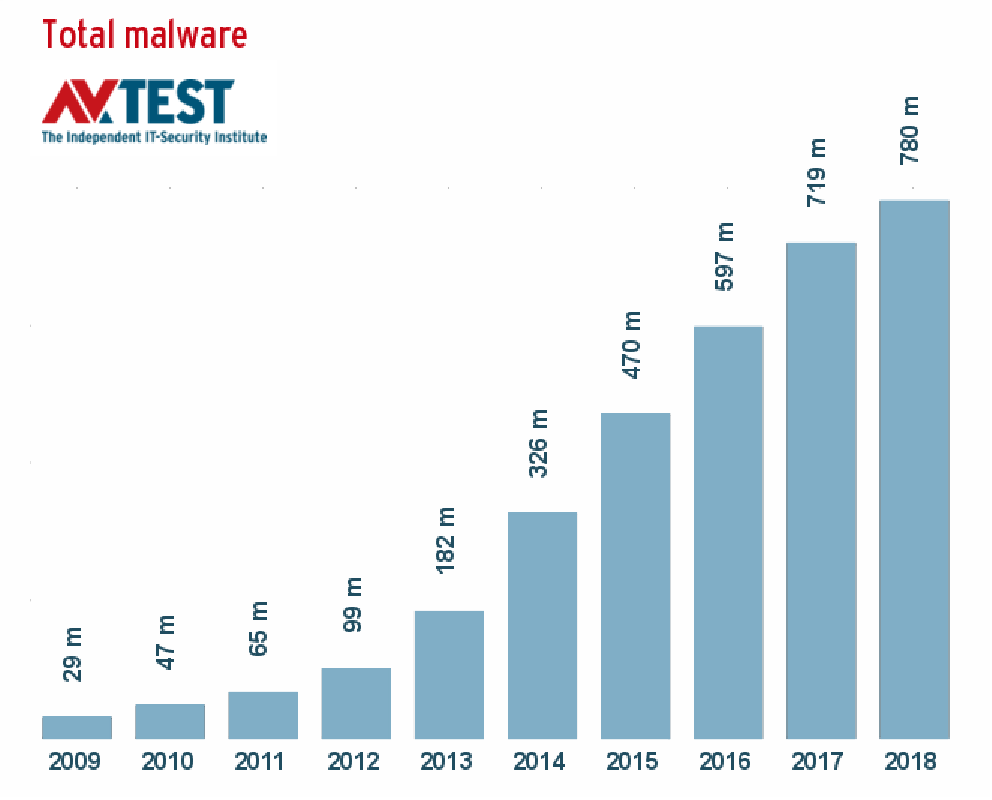
\includegraphics[scale=0.55]{image/malware2}
    \end{figure}
    
\end{frame}

\begin{frame}
    \frametitle{Malware Analysis}

    Two main types:
    \medskip
    \begin{itemize}
        \item \textbf{Static Analysis:}\\
        involves the inspection of the different data and code sections of a binary
        \item \textbf{Dynamic Analysis:}\\
        the malware sample is executed and the actions it performs on the environment are observed
    \end{itemize}
    \vspace{1cm}    
        
         \begin{beamerboxesrounded}[shadow=true]{}
    Dynamic analysis strongly favoured as it allows to dodge \\ code obfuscations and deal with a large number of samples
    \end{beamerboxesrounded}    

    \begin{textblock*}{2cm}(9.0cm,-6.5cm)
   
\includegraphics[width=1.2cm]{image/search.png}% use the \includegraphics command here
	\end{textblock*} 

\end{frame}

\subsection{Function Call Monitoring}
\begin{frame}
    \frametitle{Function call monitoring}

Functions can abstract
implementation details providing
a semantically richer representation of some functionality. \\\bigskip
Example:
    \begin{figure}
    	\vspace{-0.4cm}
        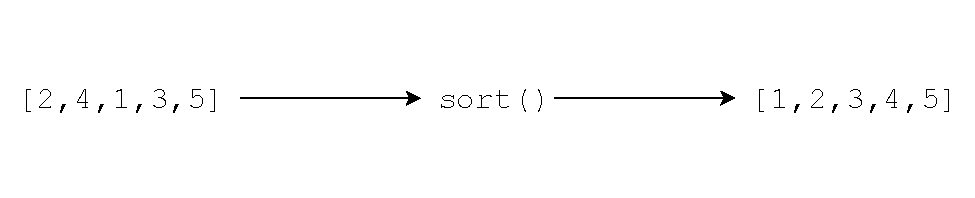
\includegraphics[scale=0.6]{image/fcmonitoring}
    \end{figure}

\begin{beamerboxesrounded}[shadow=true]{}
The abstractions embodied by \textbf{system calls} and \textbf{library calls} \\ can be used to grasp the visible behavior of a malicious sample
\end{beamerboxesrounded} 

\end{frame}

\begin{frame}
    \frametitle{Implementation of function call monitoring}
	
	    \begin{beamerboxesrounded}[shadow=true]{API Hooking}
    The interception of function calls provided by dynamically
linked \\ libraries (DLLs)
    \end{beamerboxesrounded}
    \bigskip
	Three broad categories:    
    
    \begin{itemize}
    \item Binary Rewriting
    \begin{itemize}
    \item Call Redirection
    \item Function Rewriting
    \end{itemize}
    \item Virtual Machine Introspection (VMI)
    \item \textbf{Dynamic Binary Instrumentation (DBI)}
    \end{itemize}
    
    \begin{textblock*}{2cm}(8.3cm,-3cm)
   
\includegraphics[width=2cm]{image/hook.png}% use the \includegraphics command here
	\end{textblock*} 

\end{frame}

\begin{frame}[fragile]
    \frametitle{Dynamic Binary Instrumentation (DBI)}
	
A dynamic binary analysis
technique in which the behaviour of an application is inspected at run-time via the
injection of analysis code. 
\bigskip
\begin{block}{}
\begin{lstlisting}[basicstyle=\ttfamily\large,xleftmargin=50pt]
<@\textcolor{red}{record(libcall, arg1)}@> 
retval = libcall(arg1, &arg2)
<@\textcolor{red}{record(retval, *arg2)}@> 
\end{lstlisting}
\end{block}
\bigskip
\bigskip
\textbf{Problem 1}: existing products have limited logging capabilites

\end{frame}

\subsection{Evasion}

\begin{frame}
    \frametitle{The threat posed by evasive malware}
	
		    \begin{beamerboxesrounded}[shadow=true]{Evasive malware}
Malware that conceals its harmful behaviour when detecting a
hostile environment, such as a well-known sandbox
solution
    \end{beamerboxesrounded}
    \bigskip
    
    \begin{figure}
    	\vspace{-0.2cm}
    	\hspace*{1cm}
        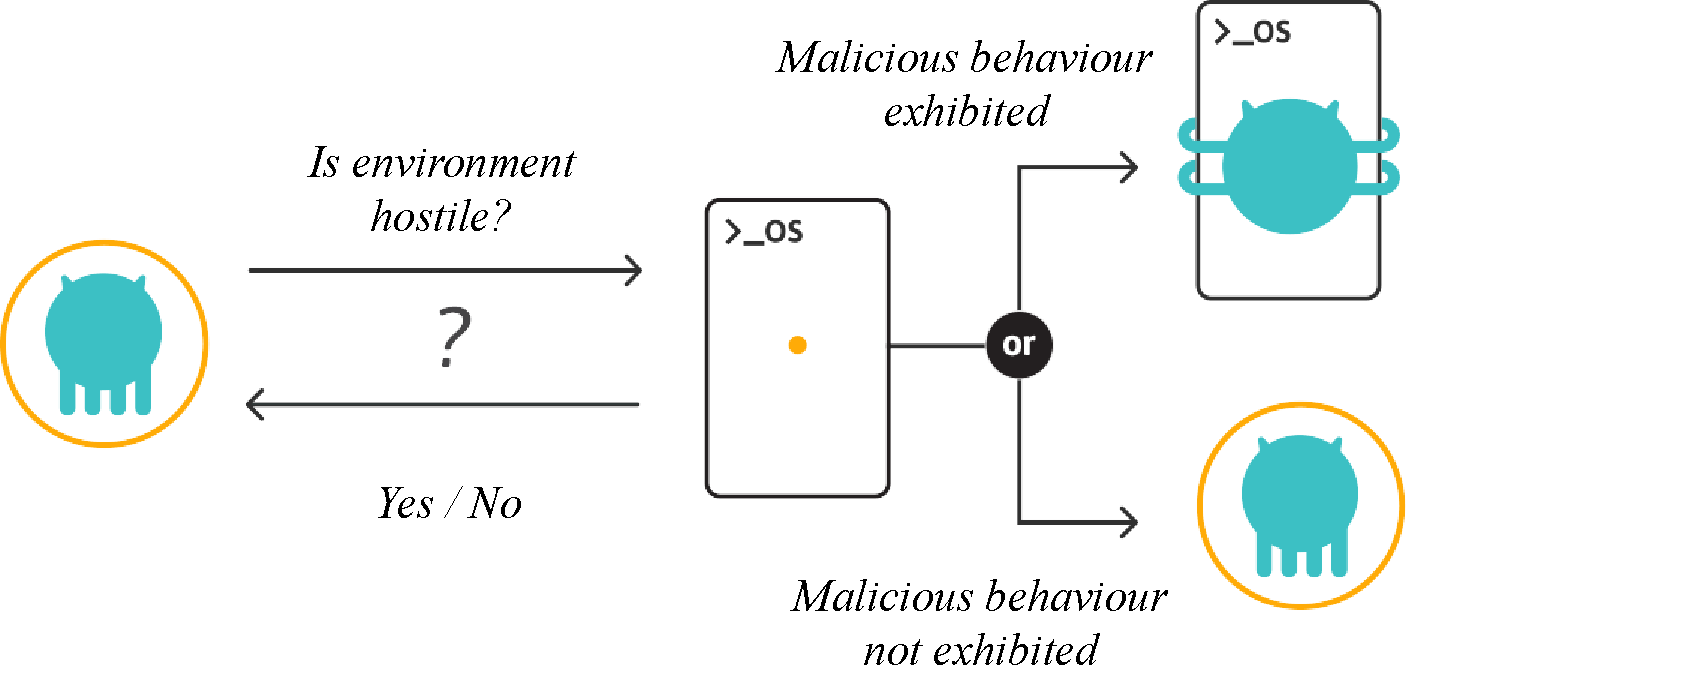
\includegraphics[width=9cm]{image/evasive.pdf}
    \end{figure}
    
    \textbf{Problem 2}: API hooking techniques in literature are not coupled with mechanisms to hide their presence from evasive malware


\end{frame}

\section{BlueTracer}

\begin{frame}
    \frametitle{Our solution: BlueTracer}

\begin{beamerboxesrounded}[shadow=true]{}
\textbf{BlueTracer} is a robust library and system call tracer for Windows programs specialized in evasive malware
\end{beamerboxesrounded}

\bigskip

Implementation details:
\begin{itemize}
\item Based on the \textbf{Intel Pin} DBI framework
\item Integrated with the \textbf{BluePill} stealthy execution framework
\item Combines reliable external sources of prototypes information
\end{itemize}

\bigskip

Key features:
\begin{itemize}
\item Undetected tracing of input parameters, output buffers and return values of over 17 000 system calls and library calls
\item Logging of asynchronous events
\item Resolution of named constants
\end{itemize}

\end{frame}

\subsection{Intel Pin}

\begin{frame}
    \frametitle{Why Intel Pin ?}
    
	Characteristics:
	\begin{itemize}
	\item \textbf{User-friendliness}
	\item \textbf{Portability}
	\item \textbf{Transparency}
	\item \textbf{Efficiency}
	\end{itemize}
	\bigskip
	\textbf{Analysis routines:} embody the code to be inserted during the application's execution\\
	\smallskip
	\textbf{Instrumentation routines:} determine where the analysis code has to be placed\\
	\bigskip
	Different analysis and instrumentation granularities
	\begin{itemize}
	\item Instruction, trace, routine and image
	\end{itemize}
    
    \begin{textblock*}{3cm}(6cm,-6.5cm)
   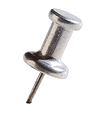
\includegraphics[width=1.6cm]{image/pin.png}% use the \includegraphics command here
	\end{textblock*}
	
	

\end{frame}

\subsection{BluePill}

\begin{frame}
    \frametitle{Integration with BluePill}
	\textbf{BluePill} is a software toolkit which:
	\begin{itemize}
	\item Allows the simulation of a real production environment a specific malware
sample was intended for
	\item Conceals any virtualization artifacts and software setup which might set off
evasion
	\end{itemize}
	\medskip
	
	    \begin{figure}
    	\vspace{-0.3cm}
    	%\hspace*{1cm}
        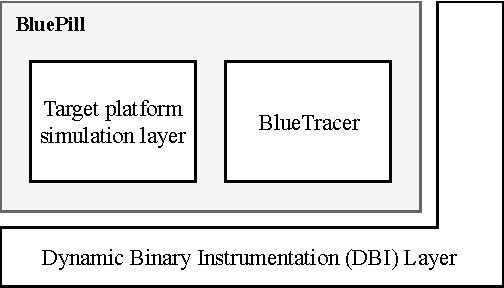
\includegraphics[width=7.5cm]{image/BluePill.pdf}
    \end{figure}

\end{frame}

\subsection{Architecture}

\begin{frame}
    \frametitle{BlueTracer's architecture}
    
    \begin{figure}
    	\vspace{-0.5cm}
    	%\hspace*{1cm}
        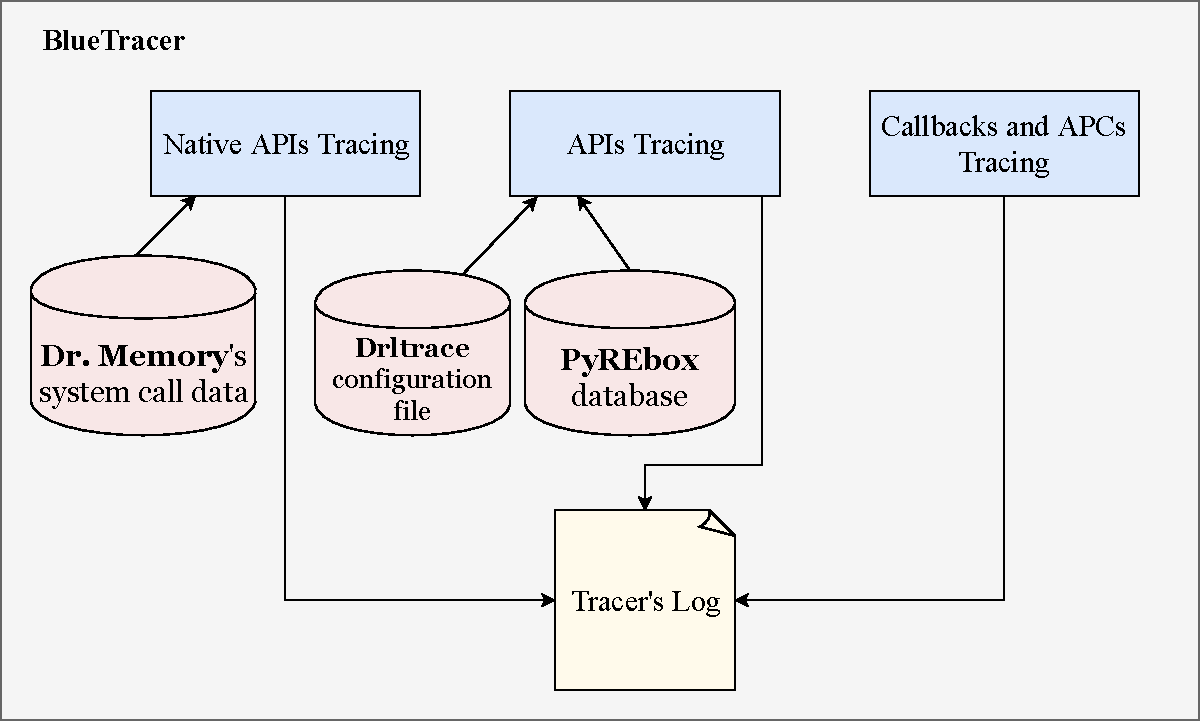
\includegraphics[width=11cm]{image/BlueTracer.pdf}
    \end{figure}
    
	

\end{frame}

\section{Evaluation}

\subsection{Al-Khaser}
\begin{frame}
    \frametitle{Evaluation with Al-Khaser}
	\textbf{Al-Khaser} is an open-source application which performs common checks employed by malware families to determine if they are being
executed in an analysis environment.
\\\medskip
Checks divided in categories:
\begin{itemize}
\item \textbf{Anti-Debugging}
\item \textbf{Timing-based}
\item \textbf{Human Interaction Detection}
\item \textbf{Anti-Virtualization}
\item \textbf{Anti-Analysis}
\end{itemize}
\bigskip
\begin{beamerboxesrounded}[shadow=true]{}
BlueTracer was undetected with respect to all the checks!
\end{beamerboxesrounded}

    \begin{textblock*}{3cm}(7.5cm,-4.cm)
   
\includegraphics[width=2cm]{image/lights.png}% use the \includegraphics command here
	\end{textblock*}

\end{frame}

\begin{frame}[fragile]
    \frametitle{Example of tracked evasion check}
    
File system artifacts can be checked in order to uncover the presence of a virtualized environment.
\vspace*{0.5cm}
    
    %\begin{figure}
    %	\vspace{-0.5cm}
    	%\hspace*{1cm}
    %    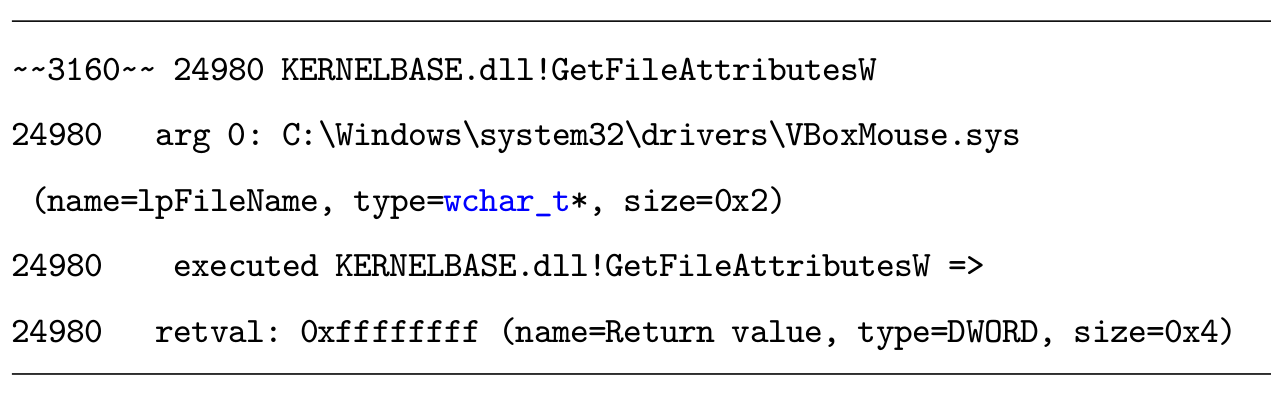
\includegraphics[width=11cm]{image/SampleCall}
    %\end{figure}
	
	\lstset{
    language=C++,
    frame=tb, % draw a frame at the top and bottom of the code block
    tabsize=4, % tab space width
    showstringspaces=false, % don't mark spaces in strings
    numbers=none, % display line numbers on the left
    commentstyle=\color{ao}, % comment color
    %keywordstyle=\color{blue}, % keyword color
    stringstyle=\color{red}, % string color
    basicstyle=\linespread{1.3}\footnotesize\ttfamily,
    basewidth = {.48em},
   escapeinside={<@}{@>}
}
\begin{lstlisting}
~~3160~~ 24980 KERNELBASE.dll!GetFileAttributesW
24980 	arg 0: <@\alert{C:Windows\textbackslash system32\textbackslash drivers\textbackslash VBoxMouse.sys}@>
 (name=lpFileName, type=wchar_t*, size=0x2)
24980    executed KERNELBASE.dll!GetFileAttributesW =>
24980 	retval: 0xffffffff (name=Return value, type=DWORD, size=0x4)
\end{lstlisting}
\lstset{
    language=C++,
    frame=tb, % draw a frame at the top and bottom of the code block
    tabsize=4, % tab space width
    showstringspaces=false, % don't mark spaces in strings
    numbers=left, % display line numbers on the left
    commentstyle=\color{ao}, % comment color
    keywordstyle=\color{blue}, % keyword color
    stringstyle=\color{red}, % string color
    basicstyle=\footnotesize\ttfamily,
    basewidth = {.48em}
} 


\end{frame}

\subsection{Evasive malware samples}
\begin{frame}
    \frametitle{Evaluation with evasive malware samples}
    
	Five highly evasive samples collected by Joe Security:    
    
    \begin{table}[h]
\vspace*{0.1cm}
\begin{center}
\resizebox{9.2cm}{!}{
 \begin{tabular}{||c c c||}
 \hline
 \textbf{ID} & \textbf{MD5} & \textbf{Name} \\ 
 \hline\hline
 1 & 0af4ef5069f47a371a0caf22ae2006a6 & \textit{trojan/banker} \\ 
 \hline
 2 & 9437eabf2fe5d32101e3fbf9f6027880 & \textit{dropper} \\
 \hline
 3 & cbdda646a20d95f078393506ecdc0796 & \textit{trojan}\\
 \hline
 4 & cfdd16225e67471f5ef54cab9b3a5558 & Olympic\\
 \hline
 5 & ef694b89ad7addb9a16bb6f26f1efaf7 & CCleaner\\ 
 \hline
\end{tabular}
}
\end{center}
\end{table}
\medskip
\begin{beamerboxesrounded}[shadow=true]{}
The
logs collected by BlueTracer reveal behaviors consistent with the analysis reports
authored by Joe Security
\end{beamerboxesrounded}	

\end{frame}

\section{Conclusions}

\begin{frame}
    \frametitle{Conclusions}
	
	\textbf{\textcolor{sapienza}{Contribution:}} \\
	\smallskip	
	\tab Design and implementation of \textbf{BlueTracer},
a robust library and system call tracer for Windows programs specialized in evasive
malware.
	\\\bigskip
	\textbf{\textcolor{sapienza}{Future Developments:}} \\
	\begin{itemize}
	\item Test with a larger set of highly evasive malware samples
	\item Improve logging capabilities
	\item Adopt log filtering techniques
	\end{itemize}

\end{frame}

\begin{frame}
\begin{center}
{\fontsize{15}{15}\selectfont \textbf{Thank you for your attention!}}
\end{center}
\end{frame}

\end{document}

